\documentclass[12pt,oneside,a4paper]{article}

\usepackage[utf8]{inputenc} % Lærer LaTeX at forstå unicode - HUSK at filen skal
% være unicode (UTF-8), standard i Linux, ikke i
% Win.

\usepackage[danish]{babel} % Så der fx står Figur og ikke Figure, Resumé og ikke
% Abstract etc. (god at have).

\usepackage{graphicx}
%\usepackage{amsfonts}
%\usepackage{esvect}
\usepackage{gensymb}

%\renewcommand{\mid}[1]{{\rm E}\!\left[#1\right]}
\newcommand{\bas}{\begin{eqnarray*}}
\newcommand{\eas}{\end{eqnarray*}}
\newcommand{\be}{\begin{equation}}
\newcommand{\ee}{\end{equation}}

\usepackage{amsthm}        % Theorems
\newtheorem{thm}{Sætning}[section]
\newtheorem{lem}{Lemma}[section]
\newtheorem{mydef}[thm]{Definition}
\newtheorem{eks}[thm]{Eksempel}

\begin{document}

\section*{Opgave}
Der er givet følgende ligning:
$$
x\sqrt{1-y^2} + y\sqrt{1-x^2} = k
$$
hvor $x$ og $y$ er reelle, og hvor $k$ er en reel konstant.

For enhver værdi af $k$ bestemmer ovenstående ligning en punkmængde i $(x,y)$ planen. Bestem denne punktmængde udtrykt med $k$.

\section*{Løsning}
Der må gælde: $-1\le x,y\le 1$. Lad nu $x=\sin(A)$ og
$y=\sin(B)$, hvor $-90\degree \le A,B \le 90\degree$.
Så har vi, at $\sqrt{1-x^2} = \cos(A)$ og $\sqrt{1-y^2} = \cos(B)$, og dermed kan ligningen skrives som:
$$
\sin(A) \cos(B) + \sin(B) \cos(A) = k
$$
Additionsformlen giver nu:
$$
\sin(A+B) = k
$$
Heraf ses tydeligt, at løsningsmængden er tom med mindre $-1\le k\le 1$. Antag derfor, at $k$ kan opfylder dette, og skriv det som 
$$
k = \sin(C)
$$
hvor $-90\degree \le C \le 90\degree$. Dermed er $\cos(C) = \sqrt{1-k^2}$.

Nu kan lignigen skrives som
$$
\sin(A+B) = \sin(C)
$$
og der er derfor to løsninger:
$$
A+B = C
$$
og 
$$
A+B = 180\degree - C
$$
Vi kan isolere $B$ is disse to løsnigner, men må samtidig tage højde for, at $B$ skal opfylde $-90\degree\le B\le 90\degree$. Det giver følgende to løsninger:
$$
B = C-A, \quad A \ge C\degree-90
$$
og
$$
B = 180\degree - C - A, \quad A \ge 90\degree-C
$$

For at vende tilbage til $(x,y)$ koordinaterne, så benytter vi nu følgende trigonometriske identitet:
$$
\sin^2(A+B) = \sin^2 (A) + \sin^2 (B) + 2\sin(A) \sin(B) \cos(A+B)
$$
Indsættes heri $\sin(A+B)=k$ og $\cos(A+B) = \pm\cos(C) = \pm\sqrt{1-k^2}$ giver dette umiddelbart:
$$
k^2 = x^2 + y^2 \pm 2xy \sqrt{1-k^2}
$$
Dette er en ellipse roteret $\pm 45\degree$ grader. Ved at indføre nye variabler:
\bas
x &=& \frac{1}{\sqrt 2} (p+q) \\
y &=& \frac{1}{\sqrt 2} (p-q)
\eas
så har vi
\bas
x^2 + y^2 &=& p^2 + q^2 \\
2xy &=& p^2 - q^2 
\eas
Dermed kan ligningen skrives som:
$$
p^2 + q^2 \pm \sqrt{1-k^2} (p^2-q^2) = k^2
$$
som kan skrives som
$$
\frac{p^2}{a^2} + \frac{q^2}{b^2} = 1
$$
hvor 
\bas
a = \frac{k}{\sqrt{1\pm\sqrt{1-k^2}}} \\
b = \frac{k}{\sqrt{1\mp\sqrt{1-k^2}}}
\eas
Læg mærke til, at $a\cdot b = k$ og $a^2 + b^2 = 2$.

I den første løsning $B = C-A, \quad A \ge C-90\degree$ skal der gælde
\bas
x &=& \sin(A) \\
  &\ge& \sin(C-90\degree) \\
  &=& -\cos(C) \\
  &=& -\sqrt{1-k^2}
\eas
I den anden løsning $B = 180\degree - C - A, \quad A \ge 90\degree-C$
skal der tilsvarende gælde: $x \ge \sqrt{1-k^2}$.

Vi har således fundet frem til følgende: For $-1\le k \le 1$ består løsningsmængden af to ellipse-udsnit. Den første har storaksen på linjen $y=-x$ og gælder i intervallet $-\sqrt{1-k^2} \le x \le 1$. Den anden har storaksen på linjen $y=x$ og gælder i intervallet $\sqrt{1-k^2} \le x \le 1$.

Den følgende figur viser løsningsmængden for $k=0.8$.

\begin{figure}[ht]
\begin{center}
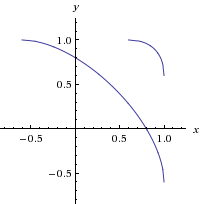
\includegraphics{opg6.png}
\label{fig1}
\end{center}
\end{figure}

\end{document}

